%\begin{frame}{Notre approche}
%Repérage des concepts dans les deux corpus en se basant sur le poids de leur apparition
%\begin{table}[!ht]
%\footnotesize
%\begin{tabularx}{\textwidth}{>{\setlength\hsize{1\hsize}\setlength\linewidth{\hsize}}X>{\setlength\hsize{1\hsize}\setlength\linewidth{\hsize}}X>{\setlength\hsize{1\hsize}\setlength\linewidth{\hsize}}X}
%\hline
%\rowcolor{blue!10}
%\multicolumn{3}{c}{Mesures de pondération}\\
%\textsc{TF-IDF} & \textsc{BM25} & \textsc{BERT} \\
%\hline
%\begin{itemize}
%    \item évalue l’importance d’un terme contenu dans
%un document relativement à un corpus plus
%large 
%    \item récompense la fréquence des
%termes et pénalise la fréquence des documents 
%\end{itemize}
%
%&
%\begin{itemize}
%    \item amélioration de \textsc{TF-IDF} 
%    \item traite les longs documents et les problèmes liés à la saturation des termes
%\end{itemize}
% &
% \begin{itemize}
%     \item modèle pré-entraîné sur de gros corpus (apprentissage non-supervisé, architecture des transformeurs)
%     \item apprend des représentations de mots et de phrases (contexte + sémantique)
%     % \item architecture des transformeurs (réseau de neurones utilisé pour le TAL)
% \end{itemize}
%\end{tabularx}
%\end{table}
%\end{frame}
\begin{frame}{OBVIE -- corpus Charcot\footnote{\url{https://obtic.huma-num.fr/obvie/charcot/?view=corpus}}}
\danger{} impossible de quantifier l'importance des phrasèmes
\begin{figure}[!h]
    \centering
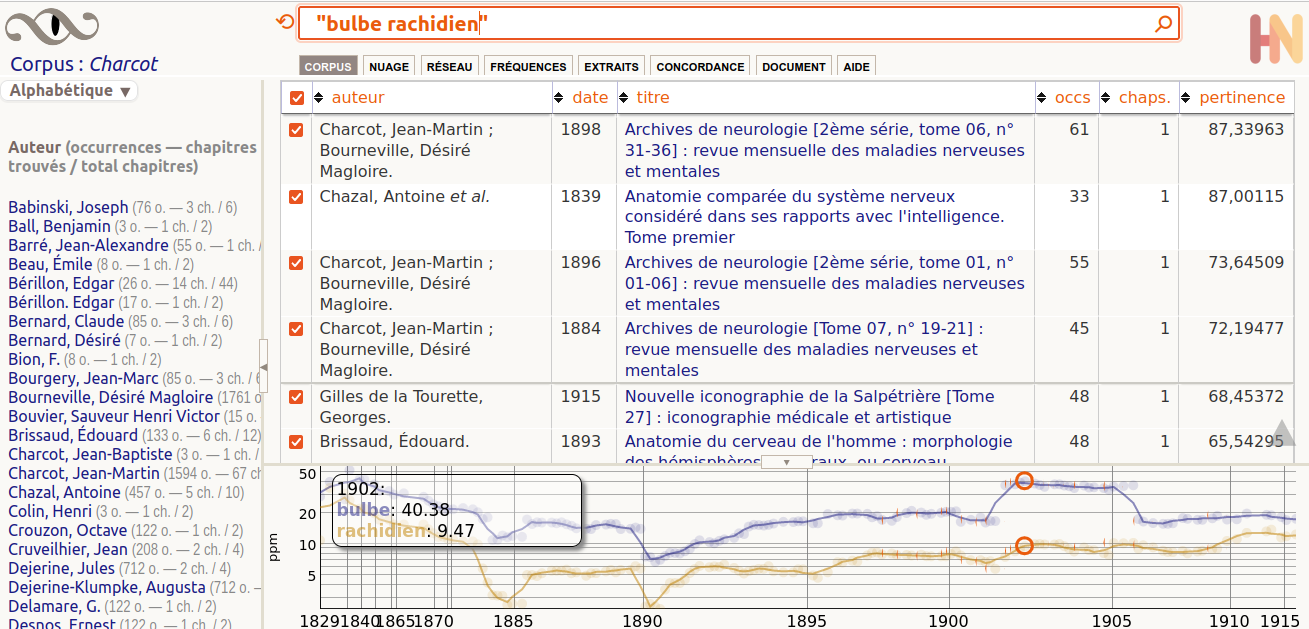
\includegraphics[width=90mm,scale=0.5]{pic/bulbe_rachidien.png}
    \caption{Distribution d'occurrences des tokens avec la frise chronologique pour ceux constituant l'expression \textit{bulbe rachidien}.}
    \label{fig:my_label}
\end{figure}
% citations directes (\cite{manjavacas2019})
\end{frame}

\begin{frame}{TextPair -- corpus Charcot\footnote{\url{https://anomander.uchicago.edu/text-pair/charcot2autres/}}}
\danger{} nombre de
résultats parfois assez conséquent $\rightarrow$ filtrage
    \begin{figure}[!ht]
        \centering
        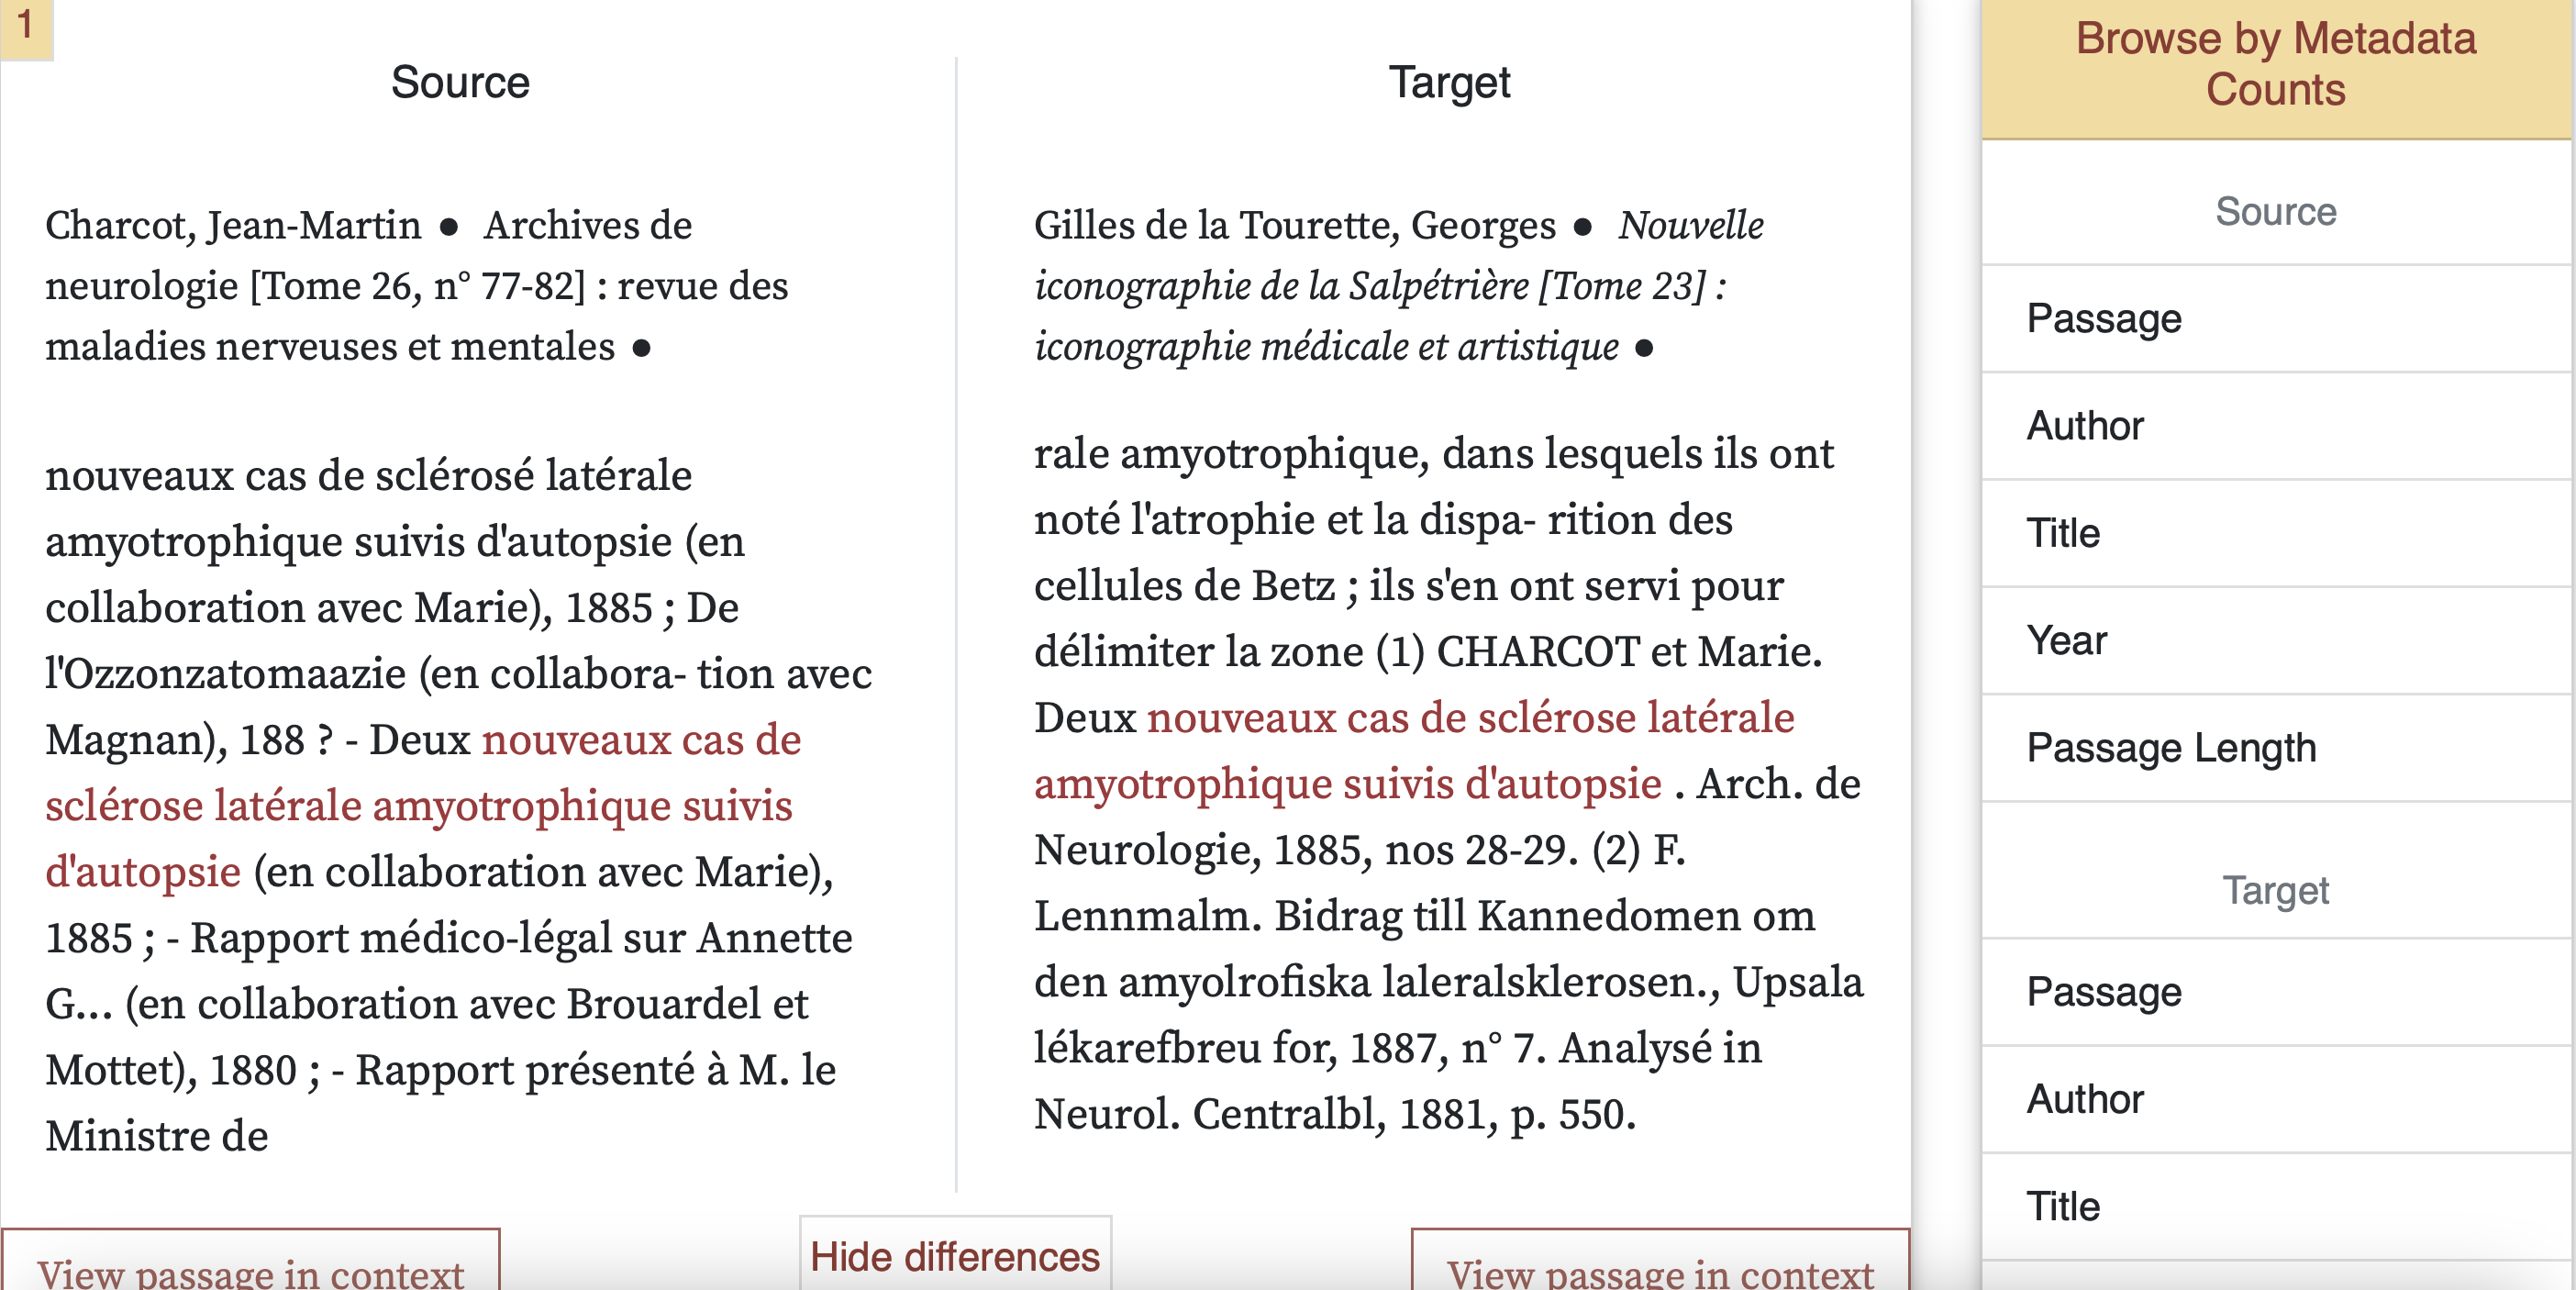
\includegraphics[width=90mm,scale=0.5]{pic/textpair.png}
        \caption{Réemploi du terme \textit{sclérose latérale amyotrophique} dans les textes de Charcot et de de la Tourette (le seul résultat).}
        \label{fig:enter-label}
    \end{figure}
\end{frame}

\begin{frame}{Liste des concepts médicaux}
    Extraction semi-automatique des termes en lien avec Charcot (\textit{hystérie}, \textit{sclérose latérale amyotrophique} etc.)
    \begin{itemize}
        \item index d’une édition des œuvres complètes de Charcot\footnote{\cite{charcot1890oeuvres}}
        \item extraction des termes à l'intérieur des balises \textsc{XML} \texttt{<s>} jusqu'à la virgule ou à un tiret avec des regex
        \item post-traitement de la liste : élimination des termes génériques (\textit{os, \textit{cerveau}, \textit{peau}, etc.})
        \item prise en compte des formes singulier / pluriel avec des regex
    \end{itemize}
\end{frame}

\begin{frame}{\textsc{TF-IDF}\footnote{angl. \textit{term frequency-inverse document frequency}.}}

\begin{block}{}
Mesure pour quantifier l'importance ou la pertinence des représentations lexicales (mots, phrases, lemmes$\dots$) dans un document parmi une collection de documents (corpus).
\end{block}
\begin{itemize}
\item \textbf{TF} : fréquence d'un terme particulier par rapport au document
\item \textbf{IDF} : calcule à quel point un terme est courant (ou rare) dans le corpus
\begin{itemize}
\item pénalise des termes fréquents et récompense les termes peu fréquents (considérés comme plus discriminants)
\end{itemize}
\end{itemize}
\end{frame}

\begin{frame}{\textsc{BM-25}\footnote{angl. \textit{best match} 25.}}

\begin{block}{}
Modèle de classement basé sur des termes qui vise à fournir des résultats de recherche précis et pertinents en classant les documents en fonction de la fréquence de leurs termes et de leur longueur.
\end{block}

\begin{enumerate}
\item TF
\item IDF
\item normalisation de la longueur de plusieurs documents
\item saturation des termes de requête
\end{enumerate}
\medskip

\color{warmblack}{TF-IDF et BM25 sont les mesures couramment utilisées dans le domaine de recherche d'information (angl. \textit{information retrieval}) 
\\$\rightarrow$ mathématiquement assez proches, surtout si appliquées sur un seul document.}

\end{frame}

\begin{frame}{Intensification du lexique
de Charcot dans le corpus \og{}Autres\fg}
\begin{figure}[!h]
    \centering
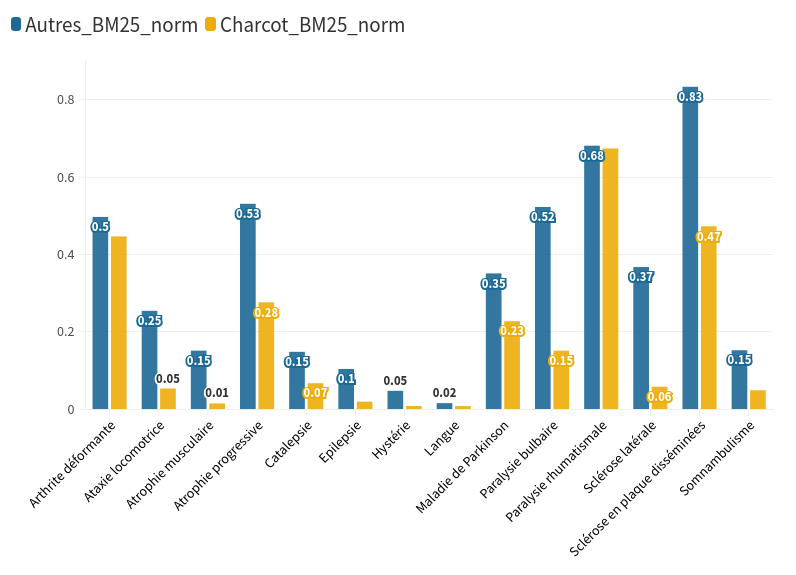
\includegraphics[width=94mm,scale=0.5]{pic/Charcot_Autres_250523.png}
    \caption{Pertinence des concepts dans les deux corpus (BM25).}
    \label{fig:my_label}
\end{figure}
\end{frame}


\begin{frame}{\textsc{BERT}}
\cite{vaswani2021}
    \begin{itemize}
        \item plongements lexicaux et des
mécanismes d’attention
        \item modèle \texttt{bert-base-multilingual-cased}
        \item censé bien capturer la sémantique
    \end{itemize}
\begin{table}[]
\begin{tabular}{ll}
\hline
Corpus \og{}Charcot\fg{}          & Corpus \og{}Autres\fg{} \\
\hline
diplopie (0,92)                & préambule (0,47)  \\
myélite partielle (0,91)       & délire (0,47)     \\
état de mal épileptique (0,91) & miracle (0,47)   \\
paralysie labio-glosso-laryngée (0,91) &
cicatrices vicieuses (0,46) \\
\textsc{pathologies} & \textsc{notions abstraites} \\
\hline 
\end{tabular}
\end{table}
\end{frame}

\begin{frame}{Calcul de pertinence des concepts : corpus \og{}Charcot\fg{}}
\footnotesize
\begin{table}[]
\begin{tabular}{|l|cccc|}
\hline
\multicolumn{1}{|c|}{{ }} &
  \multicolumn{4}{c|}{\cellcolor[HTML]{FCFF2F}{ Corpus \og{}Charcot\fg{}}} \\ \cline{2-5} 
\multicolumn{1}{|c|}{\multirow{}{}{{Terme}}} &
  {Fréquence} &
  {TF-IDF} &
  {BM25} &
  {BERT} \\ \hline
{Arthrite déformante} &
  \multicolumn{1}{|r|}{{30}} &
  \multicolumn{1}{|r|}{{0.16}} &
  \multicolumn{1}{|r|}{{0.45}} &
  {0.80} \\ \hline
{Ataxie locomotrice} &
  \multicolumn{1}{|r|}{{559}} &
  \multicolumn{1}{|r|}{{0.35}} &
  \multicolumn{1}{|r|}{{0.05}} &
  {0.83} \\ \hline
{Atrophie musculaire} &
  \multicolumn{1}{|r|}{{1 105}} &
  \multicolumn{1}{|r|}{{0.20}} &
  \multicolumn{1}{|r|}{{0.02}} &
  {0.84} \\ \hline
{Atrophie progressive} &
  \multicolumn{1}{|r|}{{40}} &
  \multicolumn{1}{|r|}{{0.14}} &
  \multicolumn{1}{|r|}{{0.27}} &
  {0.72} \\ \hline
{Catalepsie} &
  \multicolumn{1}{|r|}{{681}} &
  \multicolumn{1}{|r|}{{\textbf{0.54}}} &
  \multicolumn{1}{|r|}{{0.07}} &
  {0.88} \\ \hline
{Épilepsie} &
  \multicolumn{1}{|r|}{{414}} &
  \multicolumn{1}{|r|}{{0.09}} &
  \multicolumn{1}{|r|}{{0.02}} &
  {0.78} \\ \hline
{Hystérie} &
  \multicolumn{1}{|r|}{{5 775}} &
  \multicolumn{1}{|r|}{{0.51}} &
  \multicolumn{1}{|r|}{{0.01}} &
  {0.74} \\ \hline
{Langue} &
  \multicolumn{1}{|r|}{{2 695}} &
  \multicolumn{1}{|r|}{{0.24}} &
  \multicolumn{1}{|r|}{{0.01}} &
  {0.72} \\ \hline
{Maladie de Parkinson} &
  \multicolumn{1}{|r|}{{75}} &
  \multicolumn{1}{|r|}{{0.21}} &
  \multicolumn{1}{|r|}{{0.23}} &
  {0.81} \\ \hline
{Paralysie bulbaire} &
  \multicolumn{1}{|r|}{{149}} &
  \multicolumn{1}{|r|}{{0.27}} &
  \multicolumn{1}{|r|}{{0.15}} &
  {0.89} \\ \hline
{Paralysie rhumatismale} &
  \multicolumn{1}{|r|}{{8}} &
  \multicolumn{1}{|r|}{{0.07}} &
  \multicolumn{1}{|r|}{{0.67}} &
  {0.86} \\ \hline
{Sclérose latérale} &
  \multicolumn{1}{|r|}{{445}} &
  \multicolumn{1}{|r|}{{0.30}} &
  \multicolumn{1}{|r|}{{0.06}} &
  {0.88} \\ \hline
{Sclérose en plaque disséminées} &
  \multicolumn{1}{|r|}{{45}} &
  \multicolumn{1}{|r|}{{0.25}} &
  \multicolumn{1}{|r|}{{0.47}} &
  {0.87} \\ \hline
{Somnambulisme} &
  \multicolumn{1}{|r|}{{847}} &
  \multicolumn{1}{|r|}{{0.49}} &
  \multicolumn{1}{|r|}{{0.05}} &
  {0.89} \\ \hline
\end{tabular}
\caption{Calcul de pertinence des concepts selon TF-IDF, BM25 et BERT, corpus \og{}Charcot\fg{}.}
\end{table}
\end{frame}

\begin{frame}{Calcul de pertinence des concepts : corpus \og{}Autres\fg{}}
    \footnotesize
\begin{table}[]
\begin{tabular}{|l|cccc|}
\hline
\multicolumn{1}{|c|}{{ }} &
  \multicolumn{4}{c|}{\cellcolor[HTML]{DAE8FC}{ Corpus \og{}Autres\fg{}}} \\ \cline{2-5} 
\multicolumn{1}{|c|}{\multirow{}{}{{Terme}}} &
  {Fréquence} &
  {TF-IDF} &
  {BM25} &
  {BERT} \\ \hline
{Arthrite déformante} &
  \multicolumn{1}{|r|}{{24}} &
  \multicolumn{1}{|r|}{{0.02}} &
  \multicolumn{1}{|r|}{{\textbf{0.50}}} &
  {0.40} \\ \hline
{Ataxie locomotrice} &
  \multicolumn{1}{|r|}{{169}} &
  \multicolumn{1}{|r|}{{0.08}} &
  \multicolumn{1}{|r|}{{0.25}} &
  {0.39} \\ \hline
{Atrophie musculaire} &
  \multicolumn{1}{|r|}{{1 465}} &
  \multicolumn{1}{|r|}{{0.43}} &
  \multicolumn{1}{|r|}{{0.15}} &
  {0.42} \\ \hline
{Atrophie progressive} &
  \multicolumn{1}{|r|}{{22}} &
  \multicolumn{1}{|r|}{{0.02}} &
  \multicolumn{1}{|r|}{{0.53}} &
  {0.39} \\ \hline
{Catalepsie} &
  \multicolumn{1}{|r|}{{975}} &
  \multicolumn{1}{|r|}{{0.28}} &
  \multicolumn{1}{|r|}{{0.15}} &
  {0.39} \\ \hline
{Épilepsie} &
  \multicolumn{1}{|r|}{{577}} &
  \multicolumn{1}{|r|}{{0.12}} &
  \multicolumn{1}{|r|}{{0.10}} &
  {0.41} \\ \hline
{Hystérie} &
  \multicolumn{1}{|r|}{{4 934}} &
  \multicolumn{1}{|r|}{{0.45}} &
  \multicolumn{1}{|r|}{{0.05}} &
  {0.41} \\ \hline
{Langue} &
  \multicolumn{1}{|r|}{{3 591}} &
  \multicolumn{1}{|r|}{{0.11}} &
  \multicolumn{1}{|r|}{{0.02}} &
  {0.41} \\ \hline
{Maladie de Parkinson} &
  \multicolumn{1}{|r|}{{130}} &
  \multicolumn{1}{|r|}{{0.09}} &
  \multicolumn{1}{|r|}{{0.35}} &
  {0.37} \\ \hline
{Paralysie bulbaire} &
  \multicolumn{1}{|r|}{{93}} &
  \multicolumn{1}{|r|}{{0.09}} &
  \multicolumn{1}{|r|}{{0.52}} &
  {0.40} \\ \hline
{Paralysie rhumatismale} &
  \multicolumn{1}{|r|}{{14}} &
  \multicolumn{1}{|r|}{{0.02}} &
  \multicolumn{1}{|r|}{{\textbf{0.68}}} &
  {0.44} \\ \hline
{Sclérose latérale} &
  \multicolumn{1}{|r|}{{127}} &
  \multicolumn{1}{|r|}{{0.09}} &
  \multicolumn{1}{|r|}{{0.37}} &
  {0.41} \\ \hline
{Sclérose en plaque disséminées} &
  \multicolumn{1}{|r|}{{12}} &
  \multicolumn{1}{|r|}{{0.02}} &
  \multicolumn{1}{|r|}{{\textbf{0.83}}} &
  {0.40} \\ \hline
{Somnambulisme} &
  \multicolumn{1}{|r|}{{3 410}} &
  \multicolumn{1}{|r|}{{1}} &
  \multicolumn{1}{|r|}{{0.15}} &
  {0.43} \\ \hline
\end{tabular}
\caption{Calcul de pertinence des concepts selon TF-IDF, BM25 et BERT, corpus \og{}Autres\fg{}.}
\end{table}
\end{frame}

\begin{frame}{\texttt{keybert}}
bla
\end{frame}
